\documentclass[a4paper,12pt, twoside]{article}
%\documentclass[a4paper,12pt, twoside]{book}

\usepackage[papersize={210mm,297mm},tmargin=20mm,bmargin=20mm,lmargin=20mm,rmargin=20mm]{geometry}

\usepackage[utf8]{inputenc}
%https://mirror.hmc.edu/ctan/macros/latex/contrib/babel-contrib/turkish/turkish.pdf
\usepackage[english]{babel}
%\usepackage[T1]{fontenc}

\usepackage{amsmath,amssymb,mathabx}%\for eqref
\usepackage{lscape}
\usepackage{tcolorbox}

\usepackage{hyperref}
\hypersetup{
    colorlinks,
    citecolor=black,
    filecolor=black,
    linkcolor=blue,
    urlcolor=red}
  

%%% \usepackage{svg}
%%% https://tex.stackexchange.com/questions/122871/include-svg-images-with-the-svg-package/129854
\usepackage{graphicx}
\graphicspath{ {./figurler/} }

\usepackage[colorinlistoftodos]{todonotes}
\usepackage{fancyhdr}

\usepackage{indentfirst}
%% paragraf girintisi
\setlength{\parindent}{5ex}

%% Daha sonra yazılacak kısımları not düşmek için...
\newcommand{\YAZILACAK}{{\vspace{18pt}\bf\Large \color{red} YAZILACAK}}


\pagestyle{fancy}
\fancyhf{}
\lhead{ Kuantum Fiziği }
\chead{\thepage}
\rhead{Mesut Karakoç}
\lfoot{Akdeniz Üniversitesi}
\cfoot{}
%\rfoot{BF}

\title{Akdeniz Üniversitesi\\ Fen Fakültesi - Fizik Bölümü\\FİZ319 Kuantum Fiziği Ders Notları}

\author{\setlength{\unitlength}{6mm}
\begin{picture}(10,10)
\put(1.1,0){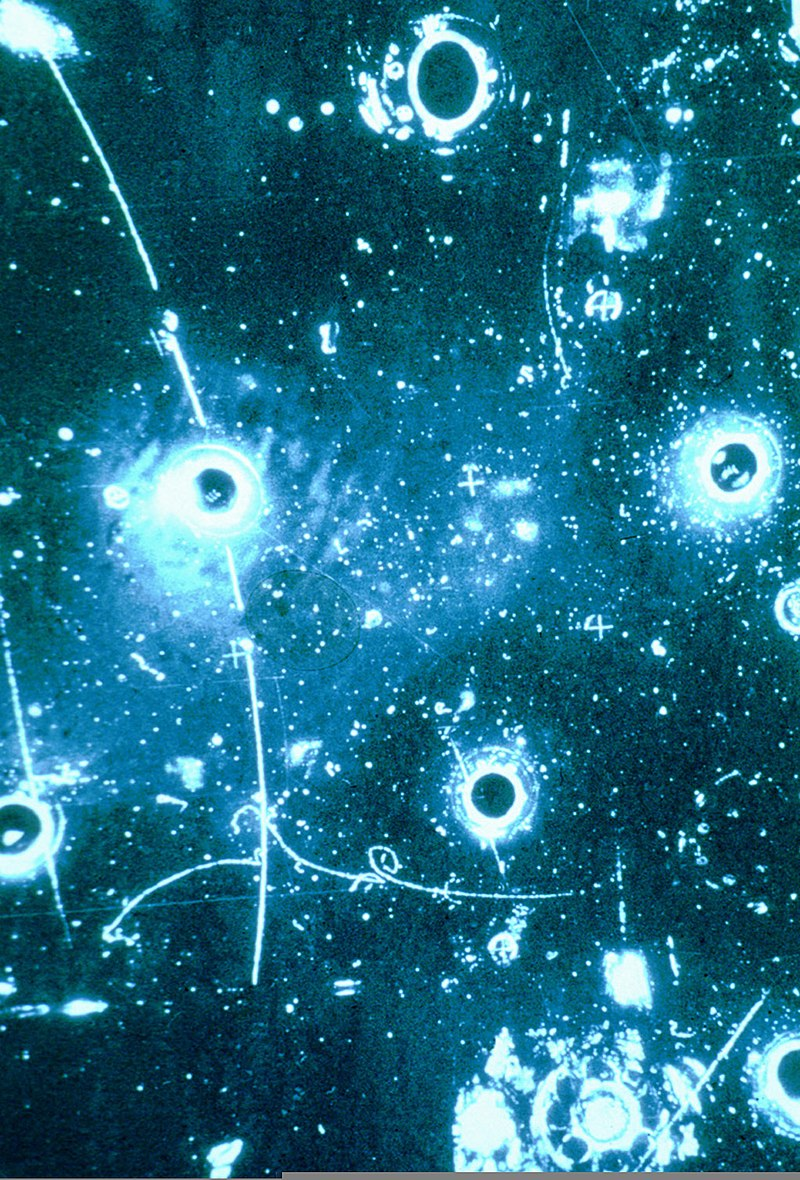
\includegraphics[width=4.5cm]{Leptonic_event_in_Gargamelle_bubble_chamber.jpg}}
\end{picture} \\ Doç. Dr. Mesut Karakoç}


\date{\today}

\begin{document}

%% Turkish babel problem
%% https://tex.stackexchange.com/questions/160385/newgeometry-doesnt-work-with-turkish-babel-package
%%\shorthandoff{=}% Make = not active any more

\maketitle

\newpage

% change name to "İçindekiler"
\renewcommand{\contentsname}{İçindekiler}
\tableofcontents{}

\listoffigures
 
\listoftables

\newpage

{
\hspace{.5\textwidth}
\begin{minipage}{.5\textwidth}
\raggedleft
If all this damned quantum jumps were really to stay, I should be
sorry I ever got involved with quantum theory.

—Erwin Schrödinger
\cite{book:Ficek}

%% Latince için
%% post iacturam quis non sapit!
%% Who is not wise after he has lost something?
%% https://quizlet.com/23756827/latin-proverbs-h-flash-cards/
\end{minipage}
}

\setcounter{section}{3} %% THIS WILL BE DELETED when all chapters merged!
\section{Bir Boyutlu Potansiyeller}

Üç boyutlu bir evrende yaşıyor olmamıza rağmen, bir çok fiziksel olayı (hareketi) bir boyutlu olarak tanımlamak mümkündür. Bu nedenle bu bölümde klasik fiziğin sınırları dışına çıkan ve kuantum fiziğiyle çalışabildiğimiz bazı bir boyutlu sistemleri inceleyeceğiz.


\subsection{Basamak Potansiyeli}
%%
\begin{figure}[hbtp]
	\centering
	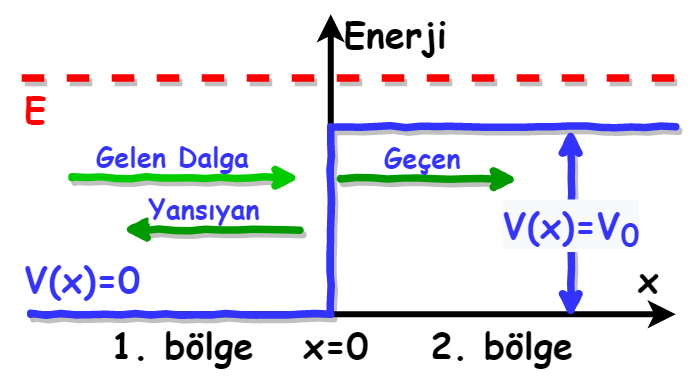
\includegraphics[width=0.6\linewidth]{figurler/Basamak_Potansiyeli.png}
	\caption{Basamak potansiyeli.}
	\label{fig:basamakpotansiyeli}
\end{figure}
%%
Bir boyutlu basamak potansiyelinin bir örneği yukarıdaki şekilde gösterilmiştir. Şekilden anlaşılacağı üzere basamak potansiyeli; birbirinden farklı sabit potansiyellere sahip iki bölgeden oluşur. Bir boyutlu bu potansiyelin matematiksel ifadesi aşağıdaki gibidir.
%%
\begin{align}
V ( x )  = \left\{ 
\begin{array} { l l } 
{ 0 } & {\Leftarrow x < 0 } \\ 
{ V _ { 0 } } & {\Leftarrow x \geq 0 } 
\end{array} \right. 
\end{align}
%%

Bu potansiyeli zamandan bağımsız Schrödinger denklemi ile çalışabiliriz. Öncelikle Schrödinger denklemini,
%%
\begin{equation}
- \frac { \hbar ^ { 2 } } { 2 m } \frac { d ^ { 2 } u ( x ) } { d x ^ { 2 } } + V ( x ) u ( x ) = E u ( x )
\end{equation}
%%
aşağıdaki gibi,
%%
\begin{equation}
\frac { d ^ { 2 } u ( x ) } { d x ^ { 2 } } + \frac { 2 m } { \hbar ^ { 2 } } [ E - V ( x ) ] u ( x ) = 0
\end{equation}
%%
yeniden yazabiliriz. Basamak potansiyelinin değerinin sıfır olduğu ve sıfırdan farklı olduğu bölgeler için, sırasıyla,
%%
\begin{equation}
\frac { 2 m} { \hbar ^ { 2 } } E \equiv k ^ { 2 } \quad \text{ ve } \quad \frac { 2 m} { \hbar ^ { 2 } }  \left( E - V _ { 0 } \right)  \equiv q ^ { 2 }
\end{equation}
%%
tanımlarını yapabiliriz. $x<0$ ve $V(x)=0$ bölgesi için çözüm
%%
\begin{equation}
u_1 ( x ) \equiv u ( x ) = A e ^ { i k x } + B e ^ { - i k x }
\end{equation}
%%
olarak yazılabilir. Burada $A e ^ { i k x }$, $x=-\infty$'deki bir kaynaktan gelen serbest düzlem dalga olarak düşünülebilir, $B e ^ { -i k x }$ ise $x=0$ noktasında ortam değişikliğinden dolayı yansıyan dalga olarak düşünülebilir. Bu bölgedeki toplam olasılık akısı,
%%
\begin{equation}
\begin{array} { r l } 
{ j_1 } &\equiv  j  = \frac { \hbar } { 2 i m } \left( u ^ { * } \frac { d u } { d x } - \frac { d u ^ { * } } { d x } u \right) \\
& = \frac { \hbar } { 2 i m } \left[ \left(A^{*} e ^ { - i k x } + B ^ { * } e ^ { i k x } \right) \left(i k A e ^ { i k x } - i k B e ^ { - i k } \right) - \left( -i k A^{*} e ^ { -i k x } + i k B^* e ^ {  i k } \right) \left( A e ^ { i k x } + B  e ^ { -i k x } \right)  \right]  \\ 
{ } & { = \frac { \hbar k } { m } \left( | A | ^ { 2 }  - | B | ^ { 2 } \right) } \end{array}
\end{equation}
%%
olur. $x>0$ ve $V(x)=V_0$ için ise,
%%
\begin{equation}
u_2 ( x ) \equiv u ( x ) =  C e ^ { i q x }
\end{equation}
%%
çözümü elde edilir. Sadece $C e ^ { i q x }$ kısmı vardır, çünkü bu bölge $x=+\infty$'a kadar uzanmaktadır ve potansiyel sabittir bu yüzden, yansıyan dalga söz konusu değildir. Sadece $+x$ yönünde ilerleyen olasılık dalgası vardır. Bu olasılık dalgası için olasılık akısı,
%%
\begin{equation}
j_2 \equiv j = \frac { \hbar q } { m } | C | ^ { 2 }
\end{equation}
%%
bulunur. Her iki bölgedeki olasılık akıları ($j_1 = j_2$) birbirine eşit olmalıdır. Eğer,
%%
\begin{equation}
\frac { \partial } { \partial t } P ( x , t ) + \frac { \partial } { \partial x } j ( x , t ) = 0
\end{equation}
%%
olduğu hatırlanırsa ve kısmi değişkenlere ayrılabilir dalga fonksiyonu ile çalıştığımızdan $P(x, t) = \psi(x,t) \psi^*(x,t) = u(x) u^*(x)$ olacağına göre,
%%
\begin{equation}\label{key}
\frac { \partial } { \partial t } P ( x , t ) = \frac { \partial } { \partial t } |u ( x)|^2 = 0
\end{equation}
%%
elde edilir. Buradan,
%%
\begin{equation}
\frac { \partial } { \partial x } j ( x , t ) = 0
\end{equation}
%%
sonucuna ulaşırız. $x=0$ civarında $x=\pm\varepsilon \rightarrow 0$ aralığında yukarıdaki ifadenin integrali,
%%
\begin{equation}
\int^{\varepsilon}_{-\varepsilon} dx \frac { \partial } { \partial x } j ( x , t ) = j (\varepsilon  , t ) - j ( -\varepsilon , t ) = 0
\end{equation}
%%
sonucunu verir. Böylece $j_1 = j_2$ olması gerektiği ortaya çıkar. Her iki bölgedeki olasılık akıları da $x$'ten bağımsız olduklarından sınırda eşitlerse bütün tanımlı uzay boyunca birbirlerine eşit olmalıdırlar,
%%
\begin{equation}
\frac { \hbar k } { m } \left( | A | ^ { 2 }  - | B | ^ { 2 } \right) = \frac { \hbar q } { m } | C | ^ { 2 }
\end{equation}
%%
yukarıdaki eşitlikle bu sonuç ifade edilmiş olur. Dalga fonksiyonlarının $x=0$'daki sürekliliğinden ise,
%%
\begin{align}
u_1(0) &= u_2(0) \\
A + B  &= C
\end{align}
%%
elde edilir. Basamak potansiyeli $x=0$'da süreksiz olmasına rağmen, sistemin dalga fonksiyonu $u(x)$ süreklidir, dalga fonksiyonun türevinin de $x=0$'da sürekli olacağı aşağıda verilen matematik süreçle gösterilmiş olur.
%%
\begin{equation}
\begin{array} { r l } { \left( \frac { d u } { d x } \right) _ { +\varepsilon } - \left( \frac { d u } { d x } \right) _ { - \varepsilon } } & { = \int _ { - \varepsilon } ^ { +\varepsilon } d x \frac { d } { d x } \frac { d u } { d x } } \\ { } & { = \int _ { - \varepsilon } ^ { +\varepsilon } d x \frac { 2 m } { \hbar ^ { 2 } } [ V ( x ) - E ] u ( x ) = 0 } \end{array}
\end{equation}
%%
Burada $\varepsilon$ sonsuz küçük bir pozitif reel sayıdır. $x=0$'ın $-\varepsilon$ ve $+\varepsilon$ civarında dalga fonksiyonlarının türevlerinin farkı yukarıdaki eşitliğin sol tarafındaki gibidir ve bu farkın integral formuda eşitliğin sağ tarafındaki gibidir. Eşitliğin sol tarafı Schrödinger denkleminden faydalanılarak $V(X)$, $E$ ve $u(x)$'i içerecek şekilde yeniden yazılabilir. Bu problemde $V(x)$ ve $E$ birer sabit sayı olduklarından, $\pm \varepsilon \rightarrow 0$ olduğundan ve böylece $u(x)$'in sürekliliği gerçekleştiğinden bu integralin cevabı sıfır olacaktır. Böylece bu tür problemler için dalga fonksiyonlarının türevlerinin de  sürekli oldukları kabul edilebilir. 

\begin{tcolorbox}
Yeri geldiğinden ve daha sonra kullanılacağı için şimdiden belirtmek gerekir ki, bu süreklilik $\lambda \delta(x-a)$ benzeri Dirac-delta fonksiyonu içeren potansiyeller için geçerli değildir. Böyle potansiyeller için süreklilik aşağıdaki gibi bir süreksizlik halini alır.
%%
\begin{equation}
\begin{aligned} \left( \frac { d u } { d x } \right) _ { a + \varepsilon } - \left( \frac { d u } { d x } \right) _ { a - \varepsilon } & = \frac { 2 m } { \hbar ^ { 2 } } \int _ { a - \varepsilon } ^ { a + \varepsilon } d x \lambda \delta ( x - a ) u ( x ) \\ & = \frac { 2 m } { \hbar ^ { 2 } } \lambda u ( a ) \end{aligned}
\end{equation}
%%
\end{tcolorbox}
	
Bu problemde türevlerinin sürekliliği sağlandığına göre; türevlerinin sürekliliğinden,
%%
\begin{align}
\frac{d}{dx}u_1(x) \bigg|_{x=0-} &= \frac{d}{dx}u_2(x) \bigg|_{x=0+} \\
i k ( A - B ) &= i q C
\end{align}
%%
elde edilir.

Bu tür problemleri çalışılırken, klasik bir dalga sisteminin davranışına benzer olarak yansıma ve geçme olasılıklarından bahsetmek mümkündür. Bu olasılıklarla ilişkili olarak, genellikle yansıma ve geçme katsayıları, sırasıyla,
%%
%%
\begin{align}
R \equiv \frac{|j_\text{yansıyan}|}{|j_\text{gelen}|} \quad \text{ ve } \quad
T \equiv \frac{|j_\text{geçen}|}{|j_\text{gelen}|}
\end{align}
%%
şeklinde tanımlanırlar. $R$ ve $T$'yi hesaplamadan önce olasılık akısı üzerinde biraz daha bilgilerimizi genişletmeliyiz: olasılık akısını üç boyutlu durum için yazacak olursak,
%%
\begin{equation}
\vec j = \frac{\hbar}{2 m i} \left[
\Psi^*(\vec r, t) \vec \nabla \Psi(\vec r, t) - 
\Psi(\vec r, t) \vec \nabla \Psi^*(\vec r, t)
\right]
\end{equation}
%%
bir vektör davranışına sahip olduğu açıkça görülür. Basamak potansiyeli probleminde, $j_1$ (1. bölgedeki olasılık akısı) aslında,
%%
\begin{equation}
\vec j_1 = \vec j_\text{gelen} + \vec j_\text{yansıyan}
\end{equation}
%%
olarak yazılabilir. $j_2$  (2. bölgedeki olasılık akısı) ise,
%%
\begin{equation}
\vec j_2 = \vec j_\text{geçen}
\end{equation}
%%
olarak yazılabilir. Akının korunumu, $\frac { \partial } { \partial x } j ( x , t ) = 0$, ise
%%
%%
\begin{equation}
\vec j_1 = \vec j_2 \quad \text{ veya } \quad \vec j_\text{gelen} + \vec j_\text{yansıyan} = \vec j_\text{geçen}
\end{equation}
%%
olmasını gerektirir. Tekrar basamak potansiyeli çalıştığımız bir boyutlu duruma döner ve vektör notasyonunu bırakırsak ve yönleri sadece $``+"$ ve $``-"$  işaretleriyle temsil edersek,
%%
\begin{equation}
j_\text{gelen} =  \frac{\hbar}{2 m i} \left[u^*_g \frac{d}{dx}u_g - u_g (\frac{d}{dx}u_g)^*\right]
\end{equation}
%%
olur. Burada $u_g = A e ^ { i k x } $ ile verilir ve $x=-\infty$'den gelen dalga fonksiyonunu temsil eder. Böylece gelen akı,
%%
\begin{equation}
j_\text{gelen} =  \frac{\hbar k}{m} |A|^2
\end{equation}
%%
olur. Benzer şekilde, yansıyan dalga $u_y = B e ^ { -i k x } $ ve geçen dalga $u_t = C e ^ { i q x } $ ifadeleri ile tanımlanırlar. Böylece yansıyan ve geçen olasılık akıları,
%%
\begin{equation}
j_\text{yansıyan} =  -\frac{\hbar k}{m} |B|^2 \quad \text{ ve } \quad
j_\text{geçen} =  \frac{\hbar q}{m} |C|^2 
\end{equation}
%%
olarak bulunurlar. Yansıma ve geçme katsayıları ise,
%%
%%
\begin{equation}
R =  \frac{|B|^2}{|A|^2} \quad \text{ ve } \quad
T =  \frac{q}{k} \frac{|C|^2}{|A|^2}
\end{equation}
%%
olarak bulunurlar. $R$ ve $T$'yi bilinmeyen $A$, $B$ ve $C$ kat sayılarından
kurtarabiliriz. Bunun için akının korunumundan ve dalga fonksiyonlarının ve türevlerinin sürekliliğinden,
%%
%%
\begin{align}
\frac { \hbar k } { m } \left( | A | ^ { 2 }  - | B | ^ { 2 } \right) &= \frac { \hbar q } { m } | C | ^ { 2 }\\
A + B  &= C \\
i k ( A - B ) &= i q C
\end{align}
%%
elde ettiğimiz yukarıdaki eşitlikleri kullanabiliriz. Olasılık akısının korunumundan elde ettiğimiz denklemin yardımıyla, kolayca,
%%
\begin{equation}
T + R =  \frac{q}{k} \frac{|C|^2}{|A|^2} + \frac{|B|^2}{|A|^2} = 1
\end{equation}
%%
olacağı gösterilebilir. Sürekliliklerden elde edilen denklemlerden de,
%%
\begin{equation}
B =  \frac{k-q}{k+q} A \quad \text{ ve } \quad
C =  \frac{2k}{k+q} A
\end{equation}
%%
olacağı gösterilebilir. Böylece $R$ ve $T$,
%%
\begin{equation}
R =  \left(\frac{k-q}{k+q}\right)^2  \quad \text{ ve } \quad
T =  \frac{4kq}{(k+q)^2}
\end{equation}
%%
olarak bulunurlar. 

$E<V_0$ durumu için dalga fonksiyonu,
%%
\begin{equation}
u ( x ) = T e ^ { - \eta x }
\end{equation}
%%
halini alır. Burada $\eta$ ($V_0>E$ olduğundan),
%%
\begin{equation}
\frac { 2 m} { \hbar ^ { 2 } }  \left(V _ { 0 } -E \right) \equiv \eta ^ { 2 }
\end{equation}
%%
olarak tanımlanır. Benzer bir matematiksel süreçten geçilerek hesaplar yapıldığında dalga fonksiyonu genlikleri arasınada,
%%
\begin{align}
%%B =  \frac{ik + \eta}{i k- \eta} A \quad \text{ ve } \quad C =  \frac{i 2k}{i k-\eta} A\\
B =  \frac{k - i \eta}{k + i \eta} A \quad \text{ ve } \quad C =  \frac{2k}{ k+i \eta} A
\end{align}
%%
ilişkileri bulunur. Olasılık akıları hesaplandında, gelen ve yansıyan akıların aynı kaldığı, fakat geçen akının sıfır olduğu görülecektir. Bu nedenle her ne kadar basamağın içine giren dalga fonksiyonunun genliği $C$ sıfır olmasa da $j_\text{geçen} = 0$ olduğundan, geçme olasılığı katsayısı,
\begin{equation}
T = \frac{|j_\text{geçen}|}{|j_\text{gelen}|} = 0
\end{equation}
%%
olur. Yansıma olasılığı katsayısı ise,
%%
\begin{equation}
R = \frac{B B^*}{A A^*} = \left(  \frac{k - i \eta}{k + i \eta} \right) \left( \frac{k + i \eta}{k - i \eta} \right)  = 1
\end{equation}
%%
olur. Aşağıdaki şekillerde $R$, $T$ ve dalga fonksiyonlarının genliklerinin $E/V_0$ oranına göre davranışları gösterilmiştir.

\begin{figure}[!hbtp]
	\begin{minipage}{.5\textwidth}
		\centering
		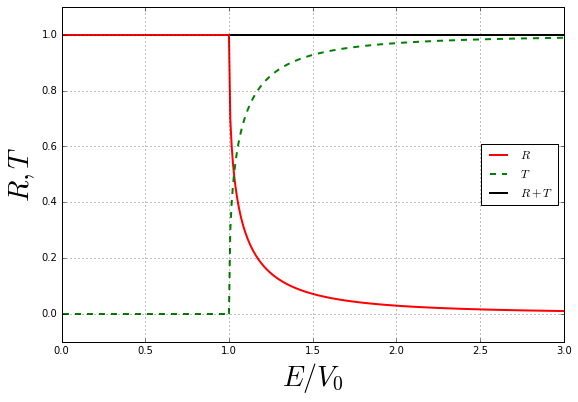
\includegraphics[width=1.0\linewidth]{Basamak_Potansiyeli_TR_EV0_grafigi.png}
		\caption{Yansıma ve geçiş katsayılarının $E/V_0$'a göre davranışları.}
		\label{fig:basamakpotansiyelitrev0grafigi}
	\end{minipage}
	\begin{minipage}{.5\textwidth}
		\centering
		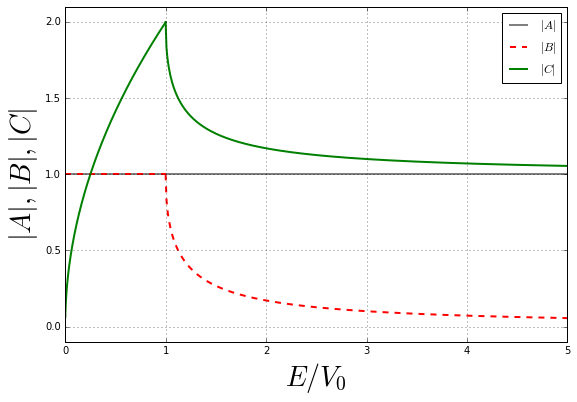
\includegraphics[width=1.0\linewidth]{Basamak_Potansiyeli_ABC_EV0_grafigi.png}
		\caption{Dalga fonksiyonu genliklerinin $E/V_0$'a göre davranışları.}
		\label{fig:basamakpotansiyeliABCev0grafigi}
	\end{minipage}
\end{figure}

Elde edilen sonuçlar hakkında bazı fiziksel yorumlar yapılabilir:
\begin{itemize}
	\item Klasik mekanik açısından bakıldığında buradaki yansıma olayı ilginçtir. Çünkü, bir potansiyelden geçen bir parçacığın kinetik enerjisini kaybedip, potansiyel enerjiye dönüştürerek, yavaşlaması beklenir. Burada gözlediğimiz yansıma davranışı ilgilendiğimiz sistemdeki parçacıkların dalga davranışı gösterdiklerini ve dalga mekaniği davranışına uygun davrandıklarını göstermektedir.
	
	\item $T + R = 1$ olması olasılık akısının korunumunun geçerliliğini onaylamaktadır. Eğer bütün parçacıkların, bütün uzay içerisinde var olma olasılığı $1$ ise yansıma ve geçme olasılıklarının toplamının $1$ olması, korunumun sağlandığını göstermektedir.
	
	\item $E>>V_0$ için $R\rightarrow0$ ve $q\rightarrow k$, bunun nedeni kolayca anlaşılabilir. Parçacığın veya sistemin enerjisi arttıkça basamak potansiyelinin etkisi neredeyse yok gibidir.
	
	\item $E<V_0$ durumu için dalga fonksiyonun $x$'in üstel azalan reel bir fonksiyonu olduğuna dikkat ediniz. Böylece $x\rightarrow+\infty$ durumunda dalga fonksiyonu ıraksamamış (patlamamış) olur. Klasik mekanikle uyumlu şekilde $R=1$ ve $T=0$ (veya ($j_\text{geçen} = 0$))olduğuna da dikkat ediniz. Fakat geçen dalganın genliği ($C\neq0$) sıfır olmamıştır (bkz. Şekil \ref{fig:basamakpotansiyeliABCev0grafigi} ) ve bu bir dalganın gösterebileceği davranıştır. Bu davranış kuantum fiziğinde \emph{``tünelleme"} olarak adlandırılır. Sonsuza uzanan basamak potansiyeli yerine sonlu kalan bir bariyer potansiyeli çalışıldığında klasik olarak yasaklı olan bölgeden bir parçacığın geçebileceği (tünelleme yapabileceği) görülecektir. 
	
\end{itemize}

\subsection{Sonlu Potansiyel Kuyusu}

\begin{figure}[hbtp]
	\centering
	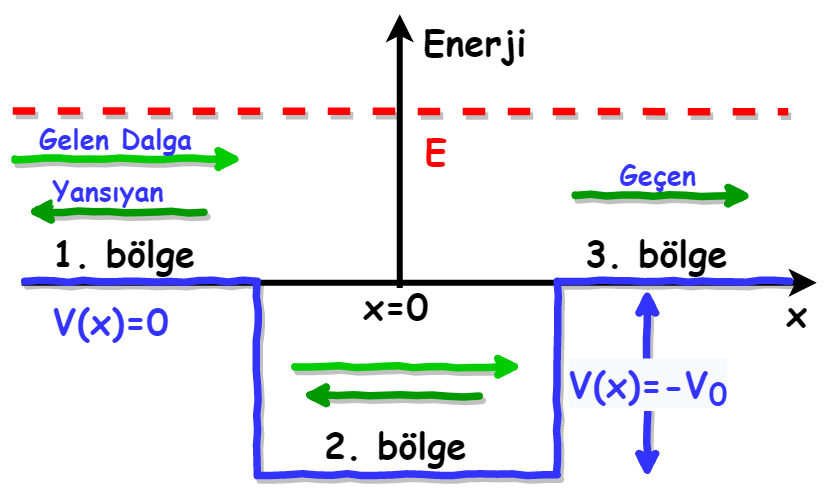
\includegraphics[width=0.62\linewidth]{figurler/SonluKuyu_Potansiyeli.png}
	\caption{Sonlu kuyu potansiyeli, $E>0$ durumu.}
	\label{fig:sonlukuyupotansiyeli}
\end{figure}

Şekil 	\ref{fig:sonlukuyupotansiyeli}'te gösterilen sonlu kuyu potansiyelinin matematik gösterimi,
%%
\begin{align}
V ( x )  = \left\{ 
\begin{array} { l l } 
{ \quad 0 } & {\Leftarrow -a > x } \\
{-V _ { 0 } } & {\Leftarrow -a \leq x \leq a } \quad \text{ (kuyunun içi)} \\
{ \quad 0 } & {\Leftarrow \quad a > x }
\end{array} \right. 
\end{align}
%%
olarak yazılabilir. Şekil incelendiğinde 1. ve 3. bölgelerde sabit ve sıfır değerli potansiyellerin, 2. bölgede ise sabit $-V_0$ değerli bir potansiyelin olduğu görülebilir.
%%
\begin{equation}
- \frac { \hbar ^ { 2 } } { 2 m } \frac { d ^ { 2 } u ( x ) } { d x ^ { 2 } } + V ( x ) u ( x ) = E u ( x )
\end{equation}
%%

Zamandan bağımsız Schrödinger denklemi bu sistem için yukarıdaki gibi olacaktır. Birinci ve üçüncü bölge için denklem,
%%
\begin{align}
\frac { d ^ { 2 } u ( x ) } { d x ^ { 2 } } +  \frac { 2 m} { \hbar ^ { 2 } } E u ( x ) = 0 \quad \text{ ve } \quad \frac { 2 m} { \hbar ^ { 2 } } E \equiv k ^ { 2 }
\end{align}
%%
ikinci bölge için ise,
\begin{align}
\frac { d ^ { 2 } u ( x ) } { d x ^ { 2 } } +  \frac { 2 m} { \hbar ^ { 2 } }  \left( E + V _ { 0 } \right) u ( x ) = 0 \quad \text{ ve } \quad \frac { 2 m} { \hbar ^ { 2 } }  \left( E + V _ { 0 } \right) \equiv q ^ { 2 }
\end{align}
%%
halini alır. Böylece bu sistemin en genel çözümü,
%%
\begin{align}
u ( x )  = \left\{ 
\begin{array} { l l } 
{u_1(x) = A_I e^{i k x} + A_R e^{-i k x} } & {\Leftarrow -a > x } \\
{u_2(x) = A e^{i q x} + B e^{-i q x} } & {\Leftarrow -a \leq x \leq a } \quad \text{ (kuyunun içi)} \\
{u_3(x) = A_T e^{i k x}} & {\Leftarrow \quad a > x }
\end{array} \right. 
\end{align}
%%
olur. Eğer çözümleri basitleştirmek için $A_I=1$ tercih edilirse, üç bölgenin olasılık akıları,
%%
\begin{align}
j ( x )  = \left\{ 
\begin{array} { l l } 
{j_1 = \frac{\hbar k}{m}\left(1-|A_R|^{2}\right) } & {\Leftarrow -a > x } \\
{j_2 = \frac{\hbar q}{m}\left(|A|^{2}-|B|^{2}\right) } & {\Leftarrow -a \leq x \leq a } \quad \text{ (kuyunun içi)} \\
{j_3 = \frac{\hbar k}{m}|A_T|^{2}} & {\Leftarrow \quad a > x }
\end{array} \right. 
\end{align}
%%
halini alırlar. Zamandan bağımsız bir davranış incelediğimizden önceki çalıştığımız sonsuz kuyu sistemine benzer şekilde olasılık akısı korunmalıdır. Böylece üç bölgenin akıları arasında,
%%
\begin{align}
	j_1 = 	j_2 = 	j_3 \Longrightarrow \frac{\hbar k}{m}\left(1-|A_R|^{2}\right)=\frac{\hbar q}{m}\left(|A|^{2}-|B|^{2}\right)=\frac{\hbar k}{m}|A_T|^{2}
	\label{eq:sonlukuyu_j1j2j3}
\end{align}
%%
eşitliği ortaya çıkar. Üç bölgenin dalga fonksiyonlarının ve türevlerinin $x=\pm$'deki değerleri, süreklilik gereğince, birbirlerine eşit olmalıdır. Buna göre türevlerden ve dalga fonksiyonlardan elde edilen denklemlerin birbirlerine oranları da, aşağıda gösterildiği gibi, birbirlerine eşit olmalıdır. 
%%
\begin{align}
\frac{1}{u_1(x)} \frac{d}{d x}u_1(x)\bigg|_{x=-a} = \frac{1}{u_2(x)} \frac{d}{d x}u_2(x)\bigg|_{x=-a}  &\Longrightarrow \frac{i q A e^{-i q a}-i q B e^{i q a}}{A e^{-i q a}+B e^{i q a}}=\frac{i k e^{-i k a}-i k A_R e^{i k a}}{e^{-i k a}+ A_R e^{i k a}} \nonumber\\
\frac{1}{u_2(x)} \frac{d}{d x}u_2(x)\bigg|_{x=+a} = \frac{1}{u_3(x)} \frac{d}{d x}u_3(x)\bigg|_{x=+a} &\Longrightarrow \frac{i q A e^{i q a}-i q B e^{-i q a}}{A e^{i q a}+B e^{-i q a}}=\frac{i k A_T e^{i k a}}{A_T e^{i k a}}=i k
\label{eq:sonlukuyu_u1u2u3}
\end{align}
%%

Denk. \ref{eq:sonlukuyu_u1u2u3}'de verilen eşitlikler ve bu eşitliklerin pay ve paydalarının ayrı ayrı eşitlikleri de kullanılarak,
%%
%\begin{align}
%{A_R=i e^{-i 2 k a} \frac{\left(q^{2}-k^{2}\right) \sin 2 q a}{2 k q \cos 2 q a-i\left(q^{2}+k^{2}\right) \sin 2 q a}} \\ 
%{A_T=e^{-i 2 k a} \frac{2 k q}{2 k q \cos 2 q a-i\left(q^{2}+k^{2}\right) \sin 2 q a}}
%\end{align}
%%
\begin{align}
{A_R= e^{-i 2 k a} \frac{\left(k^{2}-q^{2}\right) \sin 2 q a}{\left(k^{2}+q^{2}\right) \sin 2 q a + i 2 k q \cos 2 q a}} \\ 
{A_T= i e^{-i 2 k a} \frac{2 k q}{\left(k^{2}+q^{2}\right) \sin 2 q a + i 2 k q \cos 2 q a}}
\end{align}
%%
%%
yansıyan ($A_R$) ve geçen ($A_T$) dalgaların genlikleri bulunmuş olur. İncelediğimiz bu sistemi sanki $x = -\infty$'daki bir kuantum parçacığı kaynağından gelen parçacıkların sonlu kuyudan saçılması olarak düşünebiliriz. Dolayısıyla çözüm olarak önerdiğimiz dalga fonksiyonları $u_1~=~u_{gelen}~+~u_\text{yansıyan}$ ve $u_3 = u_\text{geçen}$ olarak da düşünülebilir. Bu durumda,
%%
\begin{align}
u_{gelen} &= A_I e^{i k x}, \quad j_{gelen}~=~\frac{\hbar k} {m}, \quad (A_I = 1)\\
u_\text{yansıyan} &= A_R e^{-i k x}, \quad j_\text{yansıyan} = \frac{\hbar k} {m} |A_R|^2\\
u_\text{geçen} &= A_T e^{i k x}, \quad j_\text{geçen} = \frac{\hbar k} {m} |A_T|^2
\end{align}
%%
ifadeleri ortaya çıkar. Geçiş $T$ ve yansıma $R$ katsayılarının tanımları hatırlanırsa sonlu kuyu için,
%%
\begin{align}
R &= \frac{|j_\text{yansıyan}|}{|j_\text{gelen}|} = |A_R|^2 \quad \text{(2. bölge sınırından 1. bölgeye)}\\
T &= \frac{|j_\text{geçen}|}{|j_\text{gelen}|} = |A_T|^2  \quad \text{(1. bölgeden 3. bölgeye)}
\end{align}
%%
olarak bulunurlar. Elde edilen $R$ ve $T$ katsayılarının davranışları Şekil \ref{fig:sonlukuyupot_EV0_1} ve Şekil \ref{fig:sonlukuyupot_EV0_2}'da verilmiştir. Şekil \ref{fig:sonlukuyupot_EV0_1}'te $0<E\ll V_0$ durumunda, beklendiği üzere, geçişin ($T\rightarrow0$) gittikçe azaldığı görülmektedir. Bunun aksine, Şekil \ref{fig:sonlukuyupot_EV0_2}'da $E\gg V_0>0$ durumunda, beklendiği üzere, yansımanın ($R\rightarrow0$) gittikçe azaldığı görülmektedir. Fakat her iki durumda da bazı özel enerjilerde geçisin en büyük değere ($T=1$) ve yansımanın da en düşük değere ($R=0$) ulaştığı görülmektedir. Bu özel enerjiler ``\emph{geçiş rezonansları}" olarak adlandırılan rezonans durumlarının enerjileridir. 

Bu tür saçılmalar düşük enerjili (0.1 eV) elektronların soygaz atomlardan (neon, argon v.b.) saçılması durumlarında gözlenmiştir. Bu etkiyi ilk farkedenler Ramsauer ve Towsend olmuştur \cite{book:Gasiorowicz} ve bu duruma ``\emph{geçiş rezonansları}" adını vermişlerdir. Bu rezonansları veren enerjiler $\sin(2 q a) = 0$ şartını sağlayan enerjiledir. Böylece $A_R=0$ ve dolayısıyla $R=0$ olacaktır. Bu şartı sağlayan enerjilerin,
%%
\begin{align}
E_n=-V_{0}+\frac{n^{2} \pi^{2} \hbar^{2}}{8 m a^{2}} \quad n=1,2,3, \ldots
\end{align}
%%
olacağı rahatça gösterilebilir. Şekil \ref{fig:sonlukuyupot_imU} bu tür bir rezonans enerjisinde sonlu kuyudaki dalgaların sanal kısımlarının davranışları görülmektedir. Dikkatlice bakılırsa gelen dalganın genliğinin ve fazının hiç değişmeden geçtiği kolayca görülebilir. Dolayısıyla hiç yansımanın gerçekleşmediği ve tam bir geçişin gerçekleştiği söylenebilir. Şekil \ref{fig:sonlukuyupot_u2}'da ise rezonansın gerçekleştiği enerjide dalgaların karelerinin (olasılık yoğunluklarının) davranışları verilmiştir. Bu şekilden gelen dalganın tamamen geçtiği daha açıkça anlaşılabilir. Eğer birinci bölgede yansıma sıfırdan farklı olsaydı, olasılık yoğunluğu düz bir çizgi yerine sinüssel olması (gelen ve yansıyan dalgaların tamamen yapıcı veya yıkıcı olmayan faz dışı girişimlerinden dolayı) gerekirdi.
%%
\begin{figure}[hbtp]
\begin{minipage}{.48\textwidth}
	\centering
	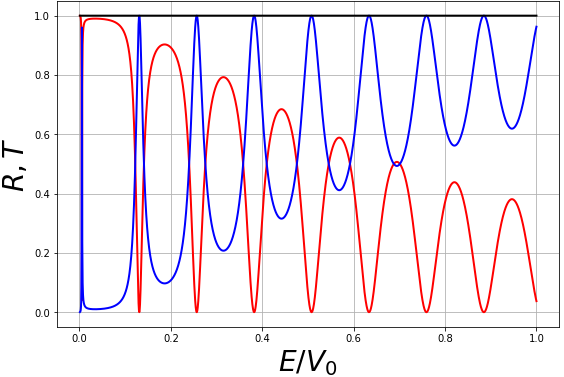
\includegraphics[width=\linewidth]{figurler/SonluKuyu_Potansiyeli_TR_EV0_1.png}
	\caption{$E/V_0 \leq 1$ durumunda $E\rightarrow0$ oldukça $T\rightarrow0$ ve $R\rightarrow1$ davranışları göstermelerine karşın, bazı özel enerji değerlerinde ($T=1$, $R=0$ olan yerlerde) ``\emph{geçiş rezonansları}" vardır.}
	\label{fig:sonlukuyupot_EV0_1}
\end{minipage}
\hspace{24pt}
\begin{minipage}{.48\textwidth}
	\centering
	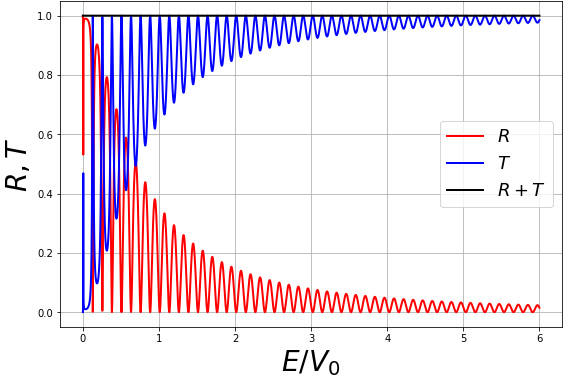
\includegraphics[width=\linewidth]{figurler/SonluKuyu_Potansiyeli_TR_EV0_2.png}
	\caption{$E/V_0\geq 1$ durumunda $T\rightarrow1$ ve $R\rightarrow0$ davranışlarını göstermektedir. Çünkü enerji arttıkça beklendiği gibi kuyunun yansıtma etkisi zayıflamaktadır.
	\vspace{12pt}}
	\label{fig:sonlukuyupot_EV0_2}
\end{minipage}
\end{figure}
%%
\begin{figure}[hbtp]
	\begin{minipage}{.48\textwidth}
		\centering
		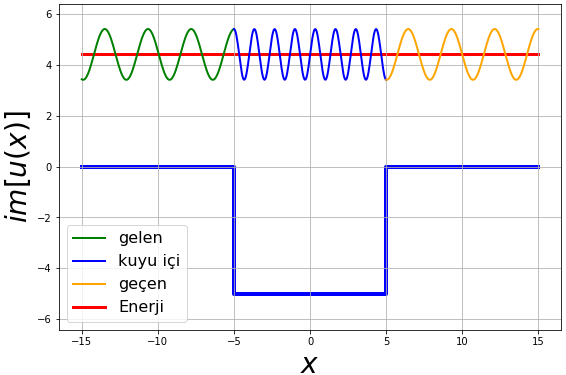
\includegraphics[width=\linewidth]{figurler/SonluKuyu_Potansiyeli_TR_imU.png}
		\caption{Şekil \ref{fig:sonlukuyupot_EV0_1}'teki $E/V_0 = 0.885$ değerinde rezonansın varlığı görülebilir. Bu değer için sonlu kuyuda gelen, geçen ve kuyu içindeki dalgaların sanal kısımlarının davranışları görülmektedir.}
		\label{fig:sonlukuyupot_imU}
	\end{minipage}
	\hspace{24pt}
	\begin{minipage}{.48\textwidth}
		\centering
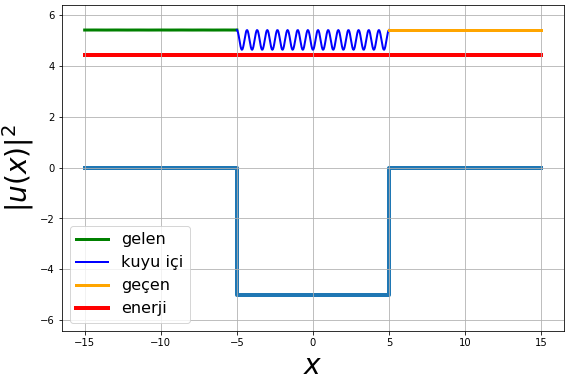
\includegraphics[width=\linewidth]{figurler/SonluKuyu_Potansiyeli_TR_u2.png}
\caption{Şekil \ref{fig:sonlukuyupot_EV0_1}'teki $E/V_0 = 0.885$ değerinde rezonansın varlığı görülebilir. Bu değer için sonlu kuyuda gelen, geçen ve kuyu içindeki dalgaların karelerinin (olasılık yoğunluklarının) davranışları görülmektedir.}
\label{fig:sonlukuyupot_u2}
	\end{minipage}
\end{figure}

Yansıma olmamasının nedeni kuyunun içindeki dalganın birden çok yansıma yapması ve bu yansımaların tekrar birinci bölgeye geçerek birinci bölgedeki yansıyan dalgayla yıkıcı girişim yapması olarak izah edilebilir. Rezonsın gerçekleşme şartının
aşağıdaki şekilde yeniden yazılmış hali optikte Fabry-Perot interferometresinin davranışını izah etmektedir \cite{book:Gasiorowicz}.
%%
\begin{align}
\lambda=\frac{2 \pi}{q}=\frac{4 a}{n}
\end{align}
%%

\subsection{Bariyer Potansiyeli}
%%
\begin{figure}[hbtp]
	\centering
	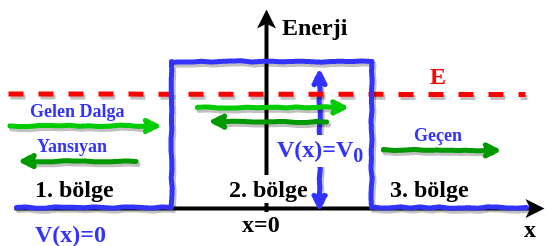
\includegraphics[width=0.62\linewidth]{figurler/Bariyer_Potansiyeli.png}
	\caption{Bariyer potansiyeli, $E<V_0$ durumu.}
	\label{fig:bariyerpotansiyeli}
\end{figure}
%%
Şekil \ref{fig:bariyerpotansiyeli}'daki bariyer potansiyeline $x=-\infty$'dan $0<E<V_0$ aralığında bir enerjiyle gelen bir kuantum nesnenin durumunu inceleyelim. Bu problemin ilginçliği: klasik olarak yasaklı olan 2. bölgeden kuantum nesnenin geçme olasılığının bulunmasıdır. Bariyer potansiyeli aşağıdaki gibi formülleştirilebilir.
%%
\begin{align}
V ( x )  = \left\{ 
\begin{array} { l l } 
{ \quad 0 } & {\Leftarrow -a > x } \\
{V _ { 0 } } & {\Leftarrow -a \leq x \leq a } \quad \text{ (bariyerin içi)} \\
{ \quad 0 } & {\Leftarrow \quad a > x }
\end{array} \right. 
\label{eq:sonlukuyupotansiyeli}
\end{align}
%%

Birinci ve üçüncü bölgelerde Schrdödinger denklemi ve çözümleri bir önceki incelediğimiz sonlu kuyu potansiyelindekilerle aynıdır. Bariyerin içinde (2. bölgede ise) Schrödinger denklemi, 
%%
\begin{equation}
- \frac { \hbar ^ { 2 } } { 2 m } \frac { d ^ { 2 } u ( x ) } { d x ^ { 2 } } + V_0 u ( x ) = E u ( x )
\end{equation}
%%
şekline sahip olur. Denklem yeniden düzenlenirse, 
%%
\begin{align}
\frac { d ^ { 2 } u ( x ) } { d x ^ { 2 } } -  \frac { 2 m} { \hbar ^ { 2 } }  \left(V _ { 0 }-E \right) u ( x ) = 0 \quad \text{ ve } \quad \frac { 2 m} { \hbar ^ { 2 } }  \left(V _ { 0 } - E \right) = q_b ^ { 2 }
\end{align}
%%
olmak üzere, 
\begin{align}
\frac { d ^ { 2 } u ( x ) } { d x ^ { 2 } } -  q_b^2 u ( x ) = 0
\end{align}
%%
halini alır. Böylece her üç bölge için dalga fonksiyonları,
%%
\begin{align}
u ( x )  = \left\{ 
\begin{array} { l l } 
{u_1(x) = A_I e^{i k x} + A_R e^{-i k x} } & {\Leftarrow -a > x } \\
{u_2(x) = A e^{- q_b x} + B e^{q_b x} } & {\Leftarrow -a \leq x \leq a } \quad \text{ (bariyerin içi)} \\
{u_3(x) = A_T e^{i k x}} & {\Leftarrow \quad a > x }
\end{array} \right. 
\end{align}
%%
olarak bulunur. Dikkat edilirse sonlu kuyu çözümleri ile bariyer çözümleri arasındaki tek fark 2. bölgede ortaya çıkmaktadır. Bu sayede sonlu kuyu için geçtiğimiz aşamalardan geçmeden,
%%
\begin{equation}
q \rightarrow i q_b = i \sqrt{\left(2 m / \hbar^{2}\right)\left(V_{0}-E\right)}
\end{equation}
%%
olacağı da göz önünde tutulursa, $A_R$ ve $A_T$ genlikleri,
%%
%%
\begin{align}
{A_R= e^{-i 2 k a} \frac{\left(k^{2}+q_b^{2}\right) \sinh 2 q_b a}{\left(k^{2}-q_b^{2}\right) \sinh 2 q_b a - 2 k q_b \cosh 2 q_b a}} \\ 
{A_T= -e^{-i 2 k a} \frac{2 k q_b}{\left(k^{2}-q_b^{2}\right) \sinh 2 q_b a - 2 k q_b \cosh 2 q_b a}}
\end{align}
%%
%%
olarak bulunurlar. Böylece, daha önce olduğu gibi yansıma ($R$) ve geçiş ($T$) katsayıları (olasılıkları),
%%
\begin{align}
R &= \frac{|j_\text{yansıyan}|}{|j_\text{gelen}|} = |A_R|^2 \quad \text{(2. bölge sınırından 1. bölgeye)}\\
T &= \frac{|j_\text{geçen}|}{|j_\text{gelen}|} = |A_T|^2  \quad \text{(1. bölgeden 3. bölgeye)}
\end{align}
%%
eşitlikleriyle hesaplanabilirler. Geçiş $T$ katsaysının açık hali,
%%
\begin{align}
T=\frac{(2 k q_b)^{2}}{\left(k^{2}+q_b^{2}\right)^{2} \sinh ^{2} 2 q_b a+(2 k q_b)^{2}}
\label{eq:bariyerpot_T}
\end{align}
%%
olarak bulunur. Yansıma katsayısı ise $R$ ise  $T+R = 1$ eşitliğinden hesaplanabilir. $T+R = 1$ olduğu birinci ve üçüncü bölgelerin akılarının eşitliklerinden rahatça ortaya konabilir. $T$ ve $R$'nin davranışları Şekil \ref{fig:bariyerpot_imU}'daki sistem için Şekil \ref{fig:bariyerpot_TR}'de çizilmiştir. Şekil \ref{fig:bariyerpot_imU}'da görüleceği üzere klasik olarak yasaklı olan ikinci bölgeden (bariyerin içinden) olasılık dalgaları geçebilmektedir. Bu nedenle $0<E<V_0$ (veya  $0<E/V_0<1$) enerjili bu olasılık dalgalarının geçiş katsayıları Şekil \ref{fig:bariyerpot_TR}'den görüldüğü üzere sıfır olmamıştır.


\begin{figure}[hbtp]
	\begin{minipage}{.48\textwidth}
		\centering
		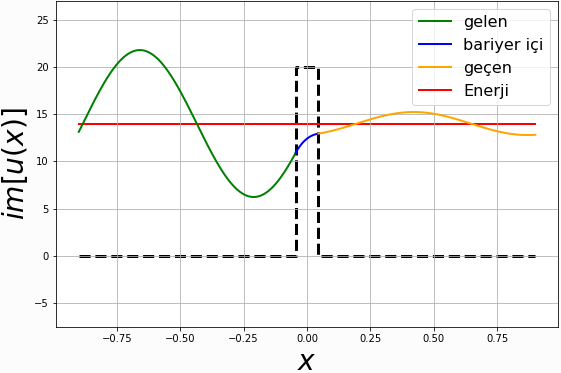
\includegraphics[width=\linewidth]{figurler/Bariyer_Potansiyeli_imU.png}
		\caption{Bir kuantum dalganın sanal kısmının bir bariyer potansiyelinden tünellemesi. Bu örnek için keyfi birimlerde: $a=0.045, E=14, V_0 = 20$ ve $\hbar = m = 1$ alınmıştır. $E/V_0 = 14/20 = 0.7$ için $T>0.8$ olduğu Şekil \ref{fig:bariyerpot_TR}'den görülebilir.
%%		\vspace{12pt}
		}
		\label{fig:bariyerpot_imU}
	\end{minipage}
	\hspace{24pt}
	\begin{minipage}{.48\textwidth}
		\centering
		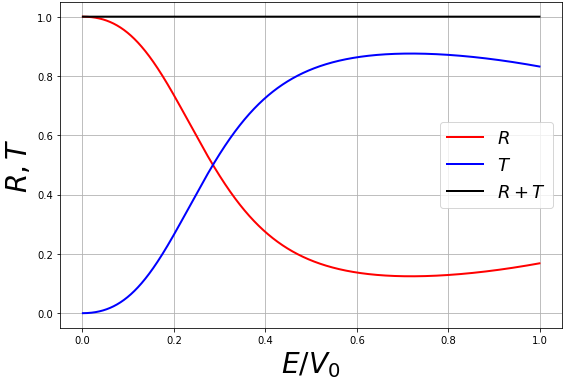
\includegraphics[width=\linewidth]{figurler/Bariyer_Potansiyeli_TR_EV0.png}
		\caption{Bu şekilde, Şekil \ref{fig:bariyerpot_imU}'daki örnek için, $0<E/V_0<1$ aralığında $R$ yansıma ve $T$ geçiş katsayılarının davranışları gösterilmektedir. Klasik fizik açısından yasaklı olan ikinci bölge için geçiş katsayısının sıfır olmadığı açıkça görülmektedir.}
		\label{fig:bariyerpot_TR}
	\end{minipage}
\end{figure}

Olasılık dalgalarının (dalga fonksiyonlarının) geçişi bariyerin genişliğine çok hassastır. 
\emph{Kalın} bir bariyer $q_b a \gg 1$ ile ifade edilebilir. Bu durumda geçiş katsayısı, 
%%
\begin{align}
T \cong\left(\frac{4 k q_b}{k^{2}+q_b^{2}}\right)^{2} e^{-2 q_b a}
\label{eq:kalinBariyer}
\end{align}
%%
halini alır. Aslında $q_b a \varpropto (V_0-E) a$ olduğunu biliyoruz. Böylece geçiş katsayısının hem bariyerin kalınlığı $a$'ya hem de bariyer potansiyelinin yüksekliği ve olasılık dalgasının enerjisi arasındaki farka hassas olduğu ortaya çıkmış oluyor. Örneğin, iki iletken tel $a = 1$~nm kalınlığında bir oksit tabaka ile ayrılmışsa ve varsayalım ki, $e^{-2 \kappa a}=10^{-10}$ olarak bulunduysa, (iletim elektronlarının yoğunluğu $10^{22}$~cm$^{-3}$ olduğundan) bir çok elektron bu oksit tabakadan geçebilir. Fakat, oksit tabakanın kalınlığı 5 kat daha fazla olsaydı ($a = 1$~nm), $e^{-2 \kappa a}=10^{-50}$ olurdu. Bu durumda efektif olarak elektronların geçişi yasaklanmış olur. Tünelleme olasılığının bu aşırı hassasiyeti taramalı tünelleme mikroskoplarının geliştirilmesini sağlamıştır \cite{book:Towsend}.

\begin{figure}[!hbtp]
		\centering
		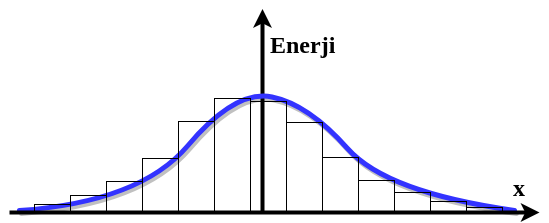
\includegraphics[width=.7\linewidth]{figurler/WKB_Bariyer_Potansiyeli.png}
		\caption{Yavaş değişen bir bariyer potansiyelinin kalın dikdörtgen bariyerler olarak yaklaşık halinin temsili.
		}
		\label{fig:yumusak_bariyerpot}
\end{figure}
%%

Çoğunlukla gerçek fiziksel sistemler keskin bir dikdörtgen bariyer şeklinde olmayabilirler. Örneğin Şekil \ref{fig:yumusak_bariyerpot}'deki gibi yavaş değişen bir potansiyel şeklinde olabilirler. Yavaş değişen bir potansiyel için Şekil \ref{fig:yumusak_bariyerpot}'te gösterildiği gibi \emph{kalın} bariyerlerden oluşan \emph{dilim}lerin toplamı gibi bir yaklaşıklık yapılabilir. Bu durumda farklı iki $k$ ve $q_b$ değilde yavaş değişen bir $q_b$ varmış gibi düşünülebilir. Böylece $q_b a \gg 1$ için ortaya çıkan Denk. \ref{eq:kalinBariyer}'teki yaklaşıklık her bir dilim için,
%%
\begin{equation}
\ln T_\text{dilim} \cong \ln \left(\frac{4 q_b k}{k^{2}+ q_b^{2}}\right)^{2}-2 q_b a \approx \mathrm{sabit}-2 q_b a
\end{equation}
%%
şeklinde yaklaşık olarak yeniden yazılabilir. Bu ifade bütün bariyer için aşağıdaki gibi yeniden yazılabilir.
%%
\begin{align} 
\ln T &=\sum_{\text {dilim }} \ln T_{\text{dilim}}=-2 \sum_{n} \Delta x_{n}\langle q_b\rangle_{n} \nonumber\\ 
&=-2 \int\limits_{\text {bariyer }} dx\sqrt{2 m(V(x)-E) / \hbar^{2}} 
\end{align}
%%
Burada $\Delta x_{n}$ her bir dilimin genişliği ve $\langle q_b\rangle_{n}$ ise dilimler için ortalama $q_b$ değeridir. Böylece yavaş değişen böyle bir potansiyel için geçiş katsayısı,
%%
\begin{equation}
T=C e^{-2 \int d x \sqrt{2 m(V(x)-E) / \hbar^{2}}}
\end{equation}
%%
ile hesaplanabilir. Bu yaklaşıklık \emph{dönüm noklarında} (enerji ve bariyer potansiyel yüksekliğinin eşit olduğu değerlerde) iyi çalışmaz. Çünkü, bu durumda, $q_b a \gg 1$ şartı altında Denk. \ref{eq:bariyerpot_T} için Denk. \ref{eq:kalinBariyer} iyi bir yaklaşık olamaz.
Bu yaklaşıklığın iyi çalışabilmesi için $V(x)$'in $x$'in yavaş değişen bir fonksiyonu olması gerektiği de unutulmamalıdır. Aksi takdirde dilimlerden oluşan yaklaşıklık ancak \emph{dar} bir bariyer potansiyeli için daha uygundur. Her ne kadar bu yaklaşıklık tünelleme olayının fiziğinin anlaşılmasına yardımcı olsa da Denk. \ref{eq:kalinBariyer} çok iyi bir yaklaşılık değildir. Daha iyi bir yaklaşıklık dönüm noktalarını da dikkate alan \emph{WKB (Wentzel–Kramers–Brillouin)} yaklaşıklığıdır.

\subsection{Kuantum Tünellemenin Uygulamaları}

Termonükleer reaksiyonlar, metaller ve yarı-iletkenlerde iletkenlik gibi
fiziksel olguların anlaşılmasında kuantum tünnelleme önemli bir yere sahiptir. 
Gamov, Condon ve Gurney kararsız ağır çekirdeklerin bünyelerinden alfa (helyum atomunun çekirdeği) parçacıkları atarak kararklı duruma geçişlerini izah edebilmişlerdir. Kurdukları modele göre alfa parçacıkları ağır çekirdeklerin içinde (proton ve nötronlara benzer şekilde) 
ağır çekirdeğin Coulomb potansiyel alanı tarafından oluşturulan bariyerden daha düşük enerjide
bulunmaktadırlar. Klasik olarak bu bariyeri aşmaları mümkün değildir. Fakat deneylerde parçacıkların ağır çekirdeklerden yayınlandığı kuantum tünelleme modeline uygun olarak gözlenmiştir. 

Ayrıca, tünelleme olgusu tünel diyodu olarak adlandırılan elektronik devre elemanının da geliştirilmesini sağlamıştır. Bu diyot akım elektronlarının enerjisinin ayarlanmasıyla bariyerin özelliklerinin değiştirilerek tünelleyen elektronların sayısının kontrol edilmesi ilkesine dayanır.

Tünellemenin en önemli uygulaması taramalı tünelleme mikroskobudur. Çok ince uçlu bir iletken yine incelenecek bir iletken yüzeye $\sim1$~nm'den daha yakın tutularak yüzeyin taranması ilkesine dayanır. İncelenecek malzemenin kendisi pozitif potansiyelde tutulursa iletken uçtaki elektronlar malzemeye geçmek isteyecektir. Fakat fotoelektrik etkiden biliyoruz ki; metallerden elektron koparabilmek için aşılması gereken bir iş fonksiyonu (potansiyeli) vardır. Dolayısıyla bu potansiyel çalıştığımız örnekte olduğu gibi tünellemesi gereken bir bariyerdir. Bu bariyerden tünelleyen elektronlar iletken uçtaki akımdaki değişimler olarak okunurlar ve böylece iletken ucun yüzeye ne kadar yakın veya uzak olduğu ölçülmüş olur. Bu sürecin terisi de mümkündür; incelenen malzeme yerine iletken uç pozitif potansiyelde tutulabilir. Sonuçta yine akımdaki değişiklikler iletken ucun malzemeye yakınlığı veya uzaklığı hakkında bilgi verecektir. Böylece malzemenin yüzeyinin haritası çıkarılmış olur \cite{book:Ficek}.

%%https://www.nanoscience.com/techniques/scanning-tunneling-microscopy/
%% https://my.eng.utah.edu/~lzang/people/zang.html
%% https://my.eng.utah.edu/~lzang/mse6075&5050-lecture-notes.html
%% https://my.eng.utah.edu/~lzang/images/Lecture_6_STM.pdf

\subsection{Sonlu Potansiyel Kuyusunda Bağlı Durumlar}

Şekil \ref{fig:sonlukuyupotansiyeli}'te gösterilen ve Denk. \ref{eq:sonlukuyupotansiyeli} ile tanımlanan sonlu potansiyel kuyusunu $E>0$ (veya saçılma) durumları için çalıştık. Bu potansiyel çekici özellikte bir kuyu şeklinde olduğundan $E<0$ durumu için ise bağlı durum çözümleri ortaya çıkacaktır. Klasik fiziktede bağlı durum potansiyelleri mevcuttur. Örneğin, güneşimiz etrafındaki gezegenler evrensel kütle çekimi ilkesince güneşin çekim potansiyeli ($-G m M/r$) altında bağlı durumda bulunurlar. Böylece kararlı Kepler yörüngelerinde güneş etrafındaki döngülerine devam ederler. Kuantum ve Klasik bağlı durumlar arasındaki en temel fark birincisinin kesikli ikincisinin sürekli enerji seviyelerine sahip olmasıdır.
%%

Zamandan bağımsız bir boyutlu Schrdinger denklemi için bağlı durum çözümleri olarak aşağıdaki dalga fonksiyonları önerilebilir.
%%
\begin{align}
u ( x )  = \left\{ 
\begin{array} { l l } 
{u_1(x) = C_1 e^{ k x} } & {\Leftarrow -a > x } \\
{u_2(x) = A \cos q x + B \sin q x } & {\Leftarrow -a \leq x \leq a } \quad \text{ (kuyunun içi)} \\
{u_3(x) = C_3 e^{- k x}} & {\Leftarrow \quad a > x }
\end{array} \right. 
\label{eq:sonlukuyubagli_df}
\end{align}
%%
Bağlı durumlarda $E<0$ durumunu çalıştığımız için enerjiyi $E = -|E|$ şeklinde göstermek daha uygun olacaktır. Böylece dalga fonksiyonlarındaki $k$ ve $q$ dalga sayıları,
%%
\begin{align}
\frac{2 m }{\hbar^{2}} |E| \equiv k^{2} \quad
\text{ ve } \quad \frac{2 m }{\hbar^{2}} (V_0-|E|) \equiv q^{2}
\end{align}
%%
olarak tanımlanabilirler. Böylece $k^2$ ve $q^2$ reel ve sıfırdan büyük değerlere sahip olurlar. Schrödinger denklemi $k^2$ ve $q^2$ ifadeleri ile yeniden yazılırsa, Denk. \ref{eq:sonlukuyubagli_df}'deki çözümler elde edilir. 

Dikkat edilirse 1. ve 3. bölge çözümleri üstel davranışlı reel dalga fonksiyonlarıdır. Bunun nedeni $E<0$ durumunda, tünelleme olayında olduğu gibi, bağlı durum dalgasının uç (kuyruk) kısımlarının duvarlardan içeri sızmasıdır. Birinci bölge için ${u_1(x) = C_1 e^{ k x} }$ seçilmiştir, çünkü $-x$ yönünde azalan bir fonksiyondur. Böylece fiziksel olmayan ve ıraksayan bir çözümden kaçınılmış olur. Benzer şekilde üçüncü bölge için ise ${u_3(x) = C_3 e^{ -k x} }$ seçilmiştir, çünkü $+x$ yönünde azalan bir fonksiyondur. İkinci bölgede ise $-V_0<E<0$ olduğundan kuantum nesnesi kuyunun içindedir, fakat kuyunun içinde kalmak şartıyla serbest dalga davranışına sahip olacaktır. Bu nedenle ikinci bölge için sinüs davranışına sahip çözümler önerilmiştir.

Bağlı durum enerji özdeğerlerini elde etmek için gerekli sınır şartlarını uygulamak isteyebiliriz. Fakat daha önce çalıştığımız sonsuz kuyu örneğinde olduğu gibi bu kuyu içinde $x\rightarrow-x$ parite dönüşümü altında $u_2(x)$'in kosinüslü kısmı \emph{çift} sinüslü kısmı ise \emph{tek} pariteye sahip olacaktır. Bu nedenle kuyunun içindeki çözümleri çift ve tek çözümler olarak ayrı ayrı çalışmak gerekir. Çift çözümler için birinci ve üçüncü bölgenin ($k^2$) kuantum özellikleri aynı olduğundan, $C_1 = C_3$ alınabilir. Tek çözümler için ise yine  her iki bölgenin kuantum özellikleri aynı fakat kuyu içindeki dalga fonksiyonu anti simetrik davranışta olduğundan, $C_1 = -C_3$ olmalıdır. $C_1$ ve $C_3$ arasındaki ilişki Şekil \ref{fig:sonlukuyu_tekcift}'ten çok daha iyi anlaşılabilir.
%%
\begin{figure}[!hbtp]
	\centering
	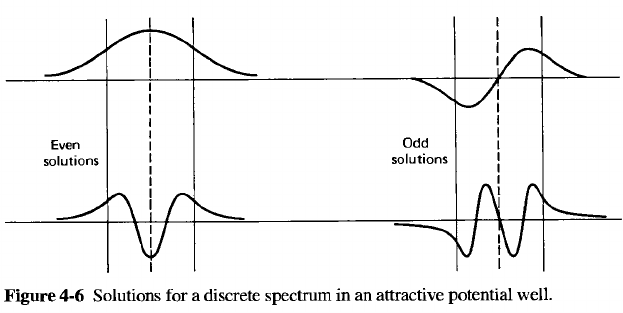
\includegraphics[width=.7\linewidth]{figurler/SonluKuyu_tek_cift_bagliDurumlar.png}
	\caption{Tek ve çift çözümler.}
	\label{fig:sonlukuyu_tekcift}
\end{figure}
%%

Önceki çalıştığımız potansiyellere benzer şekilde bu potansiyelin çözümleri olan dalga fonksiyonları ve türevleri de yine $x=\pm a$ noktasında süreklidir. Bu durumda türevlerin dalga fonksiyonlarına oranları da,
%%
\begin{equation}
\frac{1}{u(x)} \frac{d u(x)}{d x}
\end{equation}
%%
$x=\pm a$'da sürekli olacaktır. Çift çözümler için $B=0$ olmalıdır, tek çözümler için ise $A=0$ olmalıdır. Böylece çift çözümler için $u_2(x) = A \cos qx$ ve tek çözümler için $u_2(x) = B \sin qx$ olacaktır.
%%
%%
\begin{align}
\frac{1}{u(x)} \frac{d u(x)}{d x} = \left\{ 
\begin{array} { l l } 
{u_1'/u_1 = k } & \\
{u_2'/u_2 = -q\tan qx }, & \text{çift çözümler için}\\
{u_2'/u_2 = +q\cot qx }, & \text{tek çözümler için}\\
{u_3'/u_3 = -k } & 
\end{array} \right. 
\end{align}
%%
Tek ve çift çözüm durumları için elde edilen yeni süreklilik şartları $x=-a$ veya $x=+a$'da uygulanabilir. Süreklilik şartları $x=-a$'da uygulanacak olursa, çift çözümler için;
%%
\begin{align}
u_1'/u_1 = u_2'/u_2 \nonumber\\
k = -q\tan q(-a) \nonumber\\
k = q\tan q a
\end{align}
%%
tek çözümler için ise,
%%
\begin{align}
u_1'/u_1 = u_2'/u_2 \nonumber\\
k = q\cot q(-a) \nonumber\\
k = -q\cot q a
\end{align}
%%
eşitlikleri elde edilir. Elde edilen bu eşitlikler $a$ ile genişletilirse,
%%
%%
\begin{align}
\begin{array} { l l } 
ka = +qa\tan q a, & \text{çift çözümler için}\\
ka = -qa\cot q a, & \text{tek çözümler için}
\end{array}
\end{align}
%%
hallerini alırlar. Hem $k$ hem de $q$ aslında $E$'nin bir fonksiyonu olduğuna göre,


\newpage
% In the preamble, add "\renewcommand\refname{New Title}" for article type documents 
% and "\renewcommand\bibname{New Title}" for book and report type documents.
\renewcommand\refname{Kaynaklar}
\bibliography{quantumBIB}{}
%% https://www.sharelatex.com/learn/latex/bibtex_bibliography_styles
 \bibliographystyle{plain}
%% \bibliographystyle{alpha}
%%\bibliographystyle{apalike}
\end{document}

